% Chapter 1

\chapter{Intermediate version} % Main chapter title

\label{Chapter4} % For referencing the chapter elsewhere, use \ref{Chapter1} 

In this chapter the features of the intermediate version are exposed.

\section{Functional requirements}

The intermediate version (from now "gAn Web v2") is more complex than the first one. It was born from the tips and the observation of the pilot users. The modifications are not numerous, but there are a lot of additions of new features. All the new required characteristics are exposed following:

\begin{enumerate}

% 1
\item The user can insert multiple runs: separated by a semicolon (but in case of errors the system can automatically correct them replacing symbols like "-" or "," or "." with semicolons and giving a more robust service). These runs can be inserted by an input field of by a range select button: this button open a "modal" that allows the user to chose the first run and the last, and automatically insert the comprised runs (for example, if the user inserts 30000 and 30010 the system inserts automatically all the run numbers between 30000 and 30010). This modal has a validation system, that ensure the correctness of the inserted values. It is not perfectly clear if this solution fit the needs of the users, but the tests with the whole users group will probably solve this doubt. 

% 2
\item The user can chose which kind of analysis execute. At this point the different analysis are related to the different branches of gAn that at this stage an heterogeneous group of programmers are developing and uploading on Gitlab. It is no clear which of these branches will be definitive and which no, lo the program must be able to use all of them. The type of the analysis depends on the version of gAn downloaded and used for the execution of the program. In gAn Web v2 five complete branches exist, but in the future they can became more. They are externally very similar, the differences are the algorithms in the program, but they give a different output (different output but in the same format: text and images). 
At this stage is not clear if all this different versions will be used for the final application, to clarify this point the best solution is observe directly the user's behavior. 

% 3
\item The configuration file is not only in text format, but also can be in xml format (it depends on the selected version of gAn). The xml ensures a stronger structure, and must be transparent to the user (he mustn't see differences between the configurator that works with a txt file and the one that works with xml). At this stage both text format and xml format are acceptable, to ensure the retro-compatibility of some analysis, but is possible that in further versions the xml-based design will became dominant. 

%4
\item The user can chose what version of Root he wants to use for the program. Theoretically different versions of Root are perfectly compatible, but in practice each version of gAn is designed to work with a particular version of Root and to avoid problems it seems to be a good idea to allows the user to choose freely which version of Root use among the installed versions on the server.  

%5
\item The user can save images on his hard disk: he can chose from the shown images in the images page an image to download by clicking on a specific download button near the image. Furthermore there is another button "Download All" with whom the user can simple download all the output images.

%6 
\item The user can download a reduced version of the root file with informations about the images and the results: gAn produce this kind of files as "half-processed" during the computing, and it is not a problem to save this on the hard disk of the server in a specified folder. For an expert user can be scientifically interesting have this file (this root file contain more information than the output, the most of this information is useless [it is an "half-processed" file] , but sometimes an expert user can find something interesting), so the user must have the opportunity to download this.     

% 7
\item The first little group of user prefers the dropdown menu to the radio button, so all the radio buttons in the program are replaced by dropdown menus.

% 8
\item The user has to access not only to a png image, but to a root-image. This kind of image is interactive: the user can with a left click of the mouse (a continued click, like the "dragging") select parts of the image and zoom them, and with a right click do dynamically some kind of image processing (set colors, chose  what kind of chart to show, modify the chart legend, translate in a 3D space the image etcetera). In this way each user can choose freely which information he wants see in the image (try to overseen user's needs in this part seems to be too difficult and not useful).
All of this must be done by the user through a browser window. This requisite seems to be quite complex, but Root provides libraries (these libraries work well but they are poorly documented) to interact with Javascript, and can in some way resolve the problem.  

% 9
\item In the homepage the user can see the run number of the last root file produced by the machine, and its creation date and time (so, he can understand what is the maximum of the range of the insertable numbers). Also, the run number is an unit of measurement of the time, so through this number the user can have information about the progress of the experiment.  

In the intermediate version there was another functional requisite: ideally the user should have been able to select a gAn version also if not installed in the server machine: in this case the system should have been capable to automatically search on the AEgIS Gitlab repository the correct version (if existing), download it, unpack it in the server, and use it to execute the program. 
After some discussion this requirement has been cancelled, because it was considered complex, basically useless, and potentially harmful (on the branches of the repository there are untested and incomplete versions, that can create if executed wrong outputs, so wrong scientific results). At this moment installing manually the stable versions of gAn on the server seems to be a more smart way to work.

% 10
\item There is a login system: the user must insert the password of the office to use the system. The authentication is based on the confrontation between the hash function of the inserted password and the hash function of the AEgIS password. If the password is correct the user receives a cookie, before each action in the site the server request and check this cookie to be sure about the identity of the user.  


\subsection{Ambiguities (and related solutions)}

At least a point seems to be quite ambiguous: 

The textual output of gAn needs to be formatted in some way to be more organized and clear? 
The answer is difficult: for a non-physicists this output seems to be disordered, too long, with too many groups of informations, and very difficult to understand, but on this question the pilot users (that are physicists) questioned answered that the output is perfectly clear and doesn't need to be modified or improved in any way. The only requests of the users were about the font and the font-size. To check this fact the best solution probably is observe the behavior of the users at work, and eventually ask them informations about that.
Anyway, in the second version, in case of multiple run selection, there is a "navbar" that allows the user to show only a run-result per time.

\end{enumerate}


\section{Scenario based functional analysis}

Following there are a list of scenarios able to describe samples of interaction. In this situation the interaction is more complex than before.

\begin{enumerate}

\item The user wants to analyse the runs between 30000 and 30010, plus the run 31456, to make a confrontation, he is interested both in the text-output and in the images: 
the user goes to the homepage, he is redirected to the authentication page and he do the login. If successful he returns automatically in the homepage, and he can insert the runs between 30000 and 30010 manually separating them with a semicolon or better clicking the "add range of runs" button, that opens a modal, in which the user can insert the minimum and the maximum of the range, and confirm (confirmation redirects the user to the homepage). After the user can add manually the run 31456 separating it from the others with a semicolon. If the inserted run numbers make doesn't make sense the system show on the page an error message. If the inserted run numbers are valid, the user can click the "send" button (before the button was red and un-clickable, now it is green and clickable) and start gAn. A progress bar is shown, a waiting message appears, and the user waits for some seconds (at this stage of development it is very hard to predict how much time gAn requests to execute). After some seconds the user is redirected in a page that shows the textual results: on the top of the page there is a navbar that shows the computed run numbers: the user uses this navbar to chose what part of the results to show in the screen. This bar is draggable, the user can freely move it. From this page the user can, through the button "show all images", access to another page dedicated to the images. In this page he can configure through dropdown menus the dimension, the layout, the group of the images (each image belongs to a group, the group depends on the sensor that generates the data from that the image is generated) to show. He can also, by clicking on a single image, access to another page, with a single image (the clicked image) that is completely accessible: the user can rotate the image, move it in a 3d space, zoom in, zoom out, select part, do some basic digital image processing and chose the kind of chart to show.   

\item The user wants to use the version 5.34 of Root (an old but stable version) to execute gAn: 
he complete the login, in the home page there is a button name "Chose Root version", clicking on this button the user is sent to a page where, he is informed about the current version of Root, and through a dropdown menu can chose among some version of Root already installed on the server (all the acceptable Root versions are installed on the server) . If the 5.34 version is one of the installed version he can select it and confirm, the goal is achieved. If the 5.34 version is not installed, the user cannot use this version.  

\item The user wants to select the "Rug-dev" branch of gAn:
the process is very similar to the process that allows the user to chose a Root version. The user complete the login, in the home page there is a button name "Chose gAn version", clicking on this button the user is sent to a page where, he, through a dropdown menu, can chose among some branches of gAN existing on the machine. "Rug-dev" is one of these, the user can confirm and the task is completed.

\item The user wants to make the computation using only the data taken from the sensor named "Mimito":
The user, after the login, in the homepage can use the button "Edit Config" the reach a page in which, through some dropdown menus, he can change the configuration file of gAn. Each of the dropdown menus is related to a sensor (often they are 5-6, it depends on the branch), and the option of the dropdown are "yes" or "no": if "yes" is selected the sensor's data are used in the computation, if "no" they aren't. One of the dropdown menus is named "Mimito", the user select "yes" for this sensor, "no" for all the others.  

\item TODO INSERT SOMETHING RELATED TO THE ROOT LIKE IMAGE %TODO %TODO %TODO %TODO %TODO %TODO %TODO %TODO %TODO %TODO %TODO %TODO %TODO %TODO %TODO %TODO INSERT SOMETHING RELATED TO THE ROOT LIKE IMAGE

\item The user want to download all the images related to the runs 40001 and 40002:
He can, after the login, insert the runs in the homepage (it is possible both by input field and by range selector), run gAn, wait the end of the execution, click "Show all images", and from here click "download all images". All the images will be downloaded in png format. %TODO %TODO %TODO %TODO %TODO %TODO %TODO  CHECK IF THIS PROCESS IS EXACTLY similar to what is written

\item The user wants to download the semi-processed root file related to the runs 31111 and 31112:
The steps are the same as the steps used to download the images, but instead of the button "Show all images", the user has to use the button "download root files".     

\end{enumerate}  


\section{Prototypation}

The late version is based on the early version, some pages (and functionalities) are added, some existing pages are improved. 
Also in this case there aren't mock-ups, the developer chose to program directly with a common web-development process Html-javascript-php based, to optimize the time.

Following all modifications are explained.

\subsection{Modified pages}
The homepage:

\begin{figure}[H]
\centering
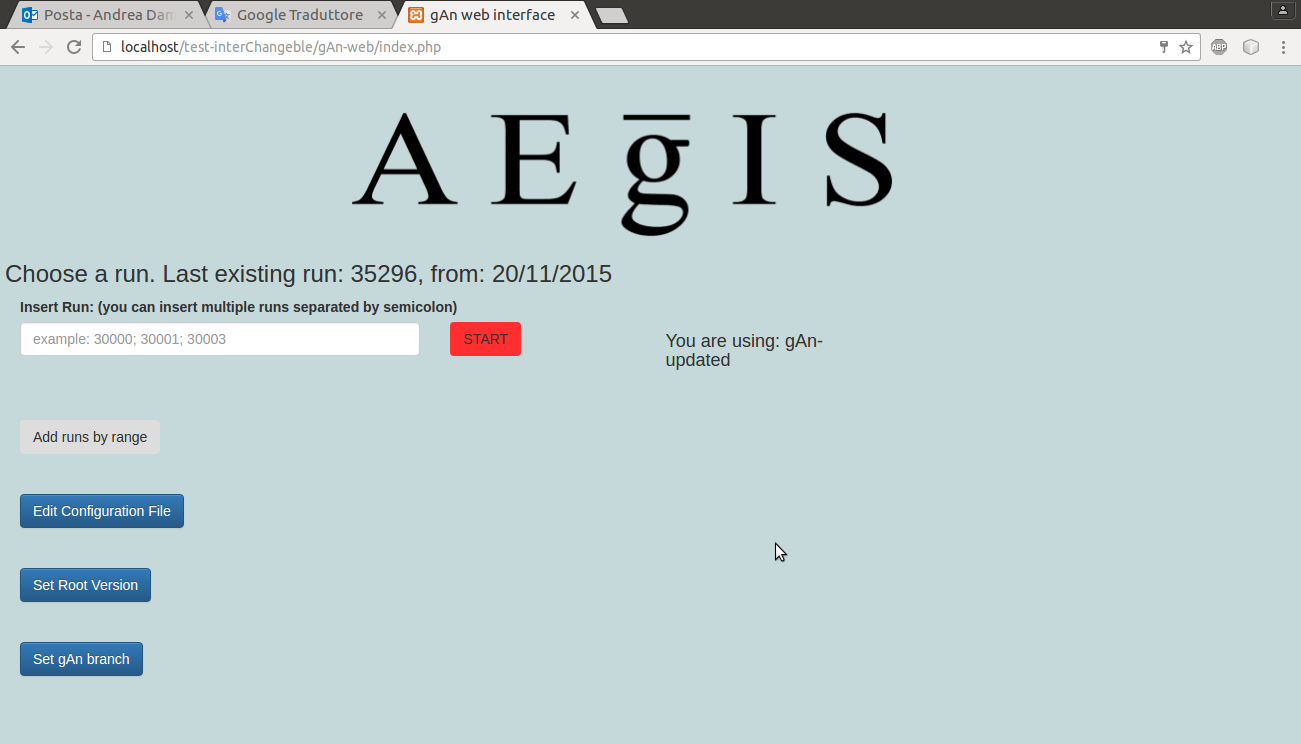
\includegraphics[scale=0.25]{HomePageEmpty.png} 
\caption{The homepage of gAn Web without input}
\end{figure}


\begin{figure}[H]
\centering
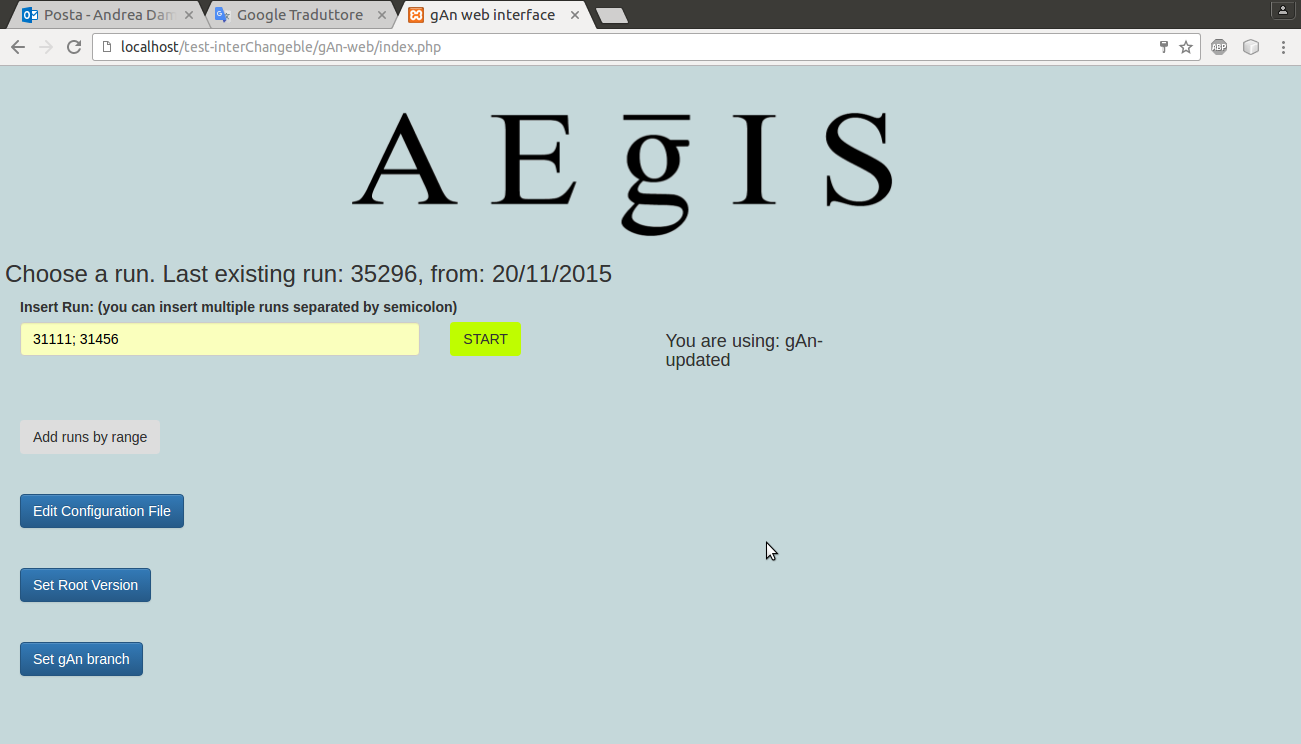
\includegraphics[scale=0.25]{HomePage.png} 
\caption{The homepage of gAn Web ready to start}
\end{figure}

There are some modifications:

\begin{enumerate}

\item The user is informed about what is the last existing run: he can read "last existing run: nnnnn, from dd/mm/yy". This point is important because in most cases the user searches results regarding the lasts 10 runs.

\item The button named "send" was unclear, the word "START" is more clear, the user can immediately understand that the goal of this button is to start gAn. The button is red and unclickable if there are problems (like in the following image) with the inserted runs (or if the input field is empty), green and clickable if there are no problems.	

\begin{figure}[H]
\centering
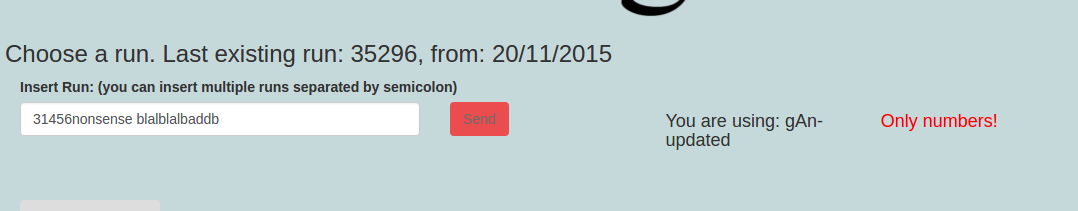
\includegraphics[scale=0.25]{ErrorInputHomepage.png}  
\caption{The "Start" button is red if the values in the input field are invalid}
\end{figure}

When the user clicks start a progress bar appears. Unfortunately it is very hard to understand exactly how long the computation will last, because different runs can take different time (it depends on the amount of data that the sensors take about the run, and on the workload of the server machine, that is in common with other applications). On average is observed that the computation take five seconds multiplied by the number of selected runs, but if another user asked for that computation before the system already has the results in memory and the computation is faster. A wait of several seconds can be not comfortable for the user, the progress bar is imprecise but ensure to the user that the system is working correctly to ensure the correct answer. In the following image the progress bar:

\begin{figure}[H]
\centering

\includegraphics[scale=0.25]{ProgressBar.png}  
\caption{The progress aimed to make more comfortable the user's waiting}
\end{figure}



\item The input field has a place-holder, that shows to the user how to correctly insert the runs separated by semicolon (there is an automatic system that corrects the inserted values if the separator is not a semicolon)
 
\item It is possible to insert a group of runs selecting them by range (inserting the first and the last): the button "Add runs by range" opens a modal (shown in the image). The user can choose the minimum and the maximum of the range, the system validates the inserted values (maximum must be more that minimum, they must be numbers etcetera).

\begin{figure}[H]
\centering
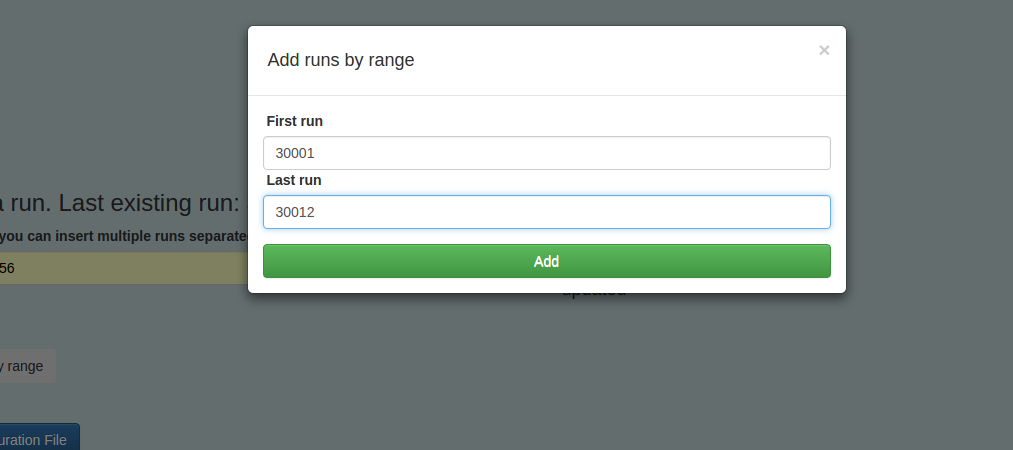
\includegraphics[scale=0.25]{RangeRunsModal.png}  
\caption{The modal opened by clicking the button "Add runs by range"}
\end{figure}

\item There is a little message "You are using: nameOfGAnBranch" that informs the user about which is the branch of gAn used by default if he doesn't change the configuration (the default branch is the last used, because usually when a group of users starts to use a branch, it continues to use it for some days)

\item There are two new buttons: "Choose Root version", "Choose gAn version". These buttons redirect the user to pages able to modify the version of Root and gAn used in the computation.
 
\item Each button and each field have a tooltip: a little explaining text that appears when the user moves the mouse over the object. In this way an inexperienced user can easily understand what each component does.  

\end{enumerate}


The page related to the modifications of the configuration file of gAn:

\begin{figure}[H]
\centering
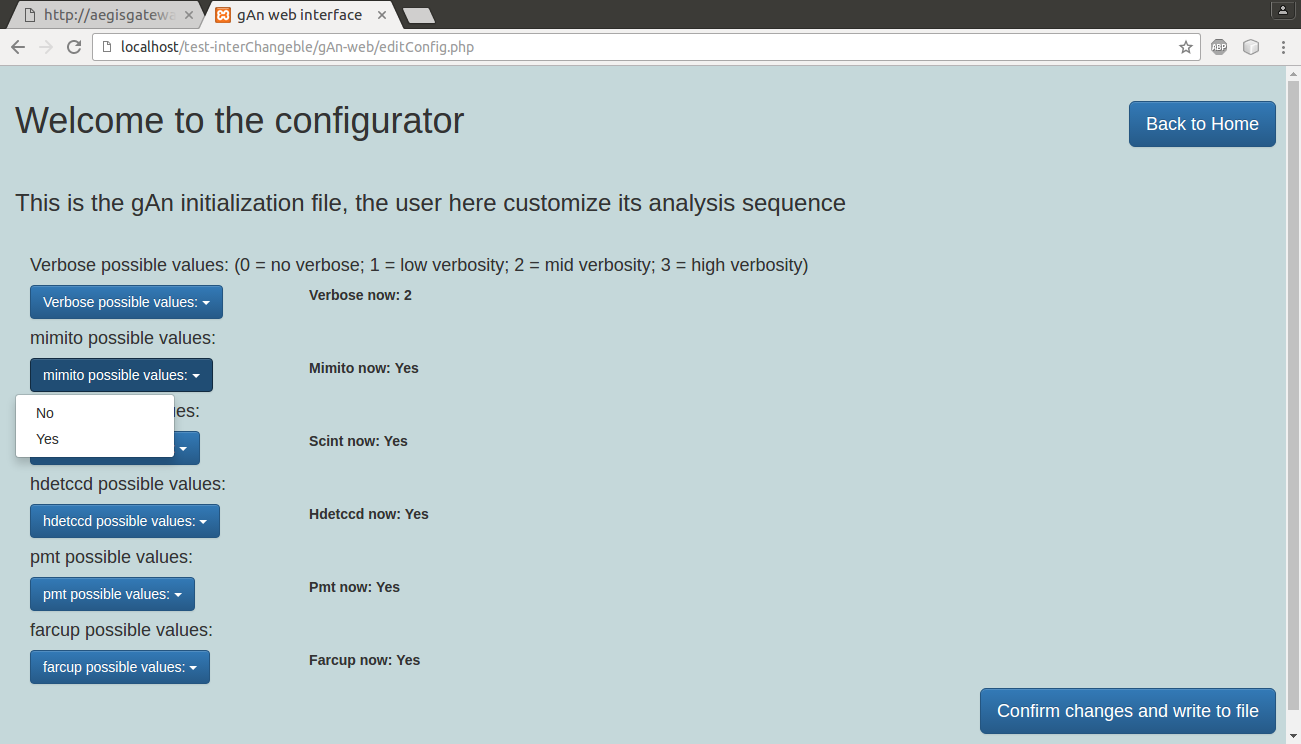
\includegraphics[scale=0.25]{EditConfig.png} 
\caption{The edit-configurator page of gAn Web}
\end{figure}

This page doesn't use anymore radio buttons, because some users ask the developers to use dropdown menus (for aesthetic reasons). The user can read near the button the currently selected value for each field. There aren't tool-tips able to describe the signification of each field here, because the users to which gAn Web is intended have a perfect understanding of the names and the features of each sensor (mimito, scint, farcup, etcetera are sensors).  



The page that shows the textual output of gAn is exposed in the following images, has some modifications:

\begin{figure}[H]
\centering
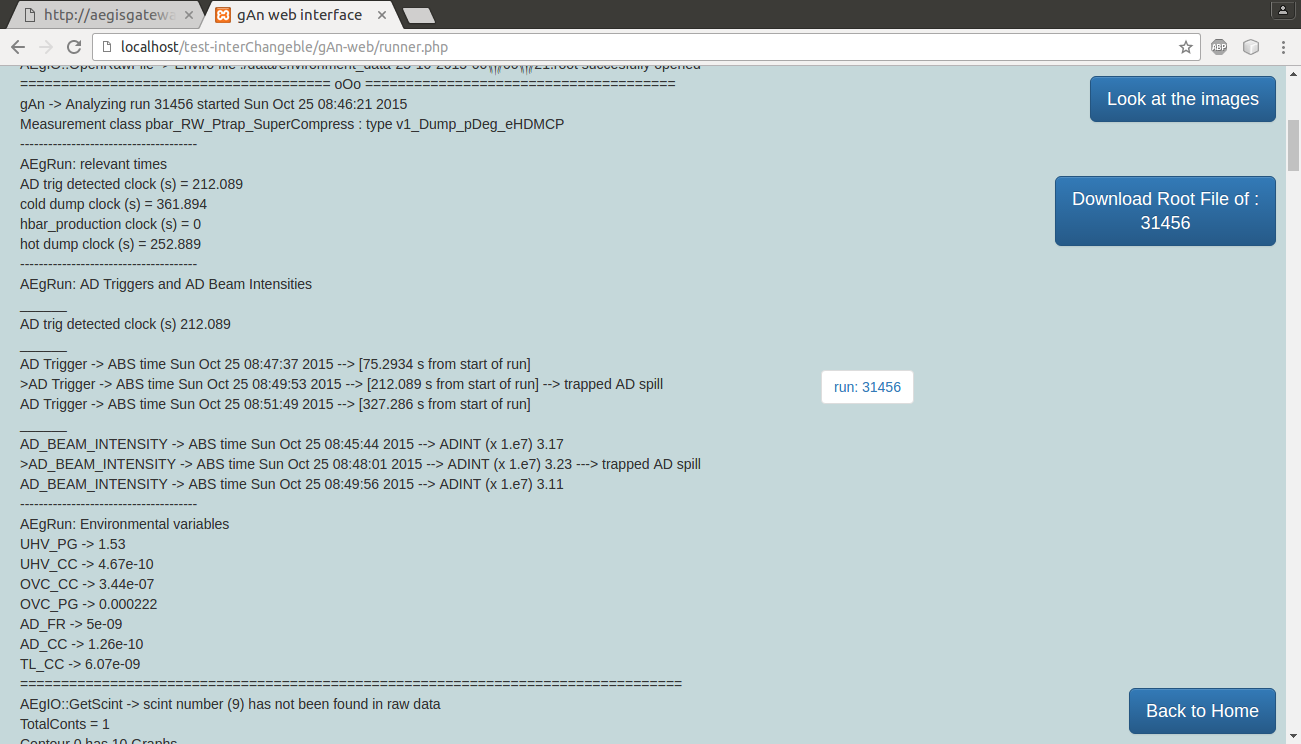
\includegraphics[scale=0.25]{TextOutputPage.png} 
\caption{The page who shows the textual output of gAn}
\end{figure}


\begin{enumerate}
\item The user can choose what results he wants to show on the screen by clicking the corresponding run number from the "navbar", like in the image:

\begin{figure}[H]
\centering
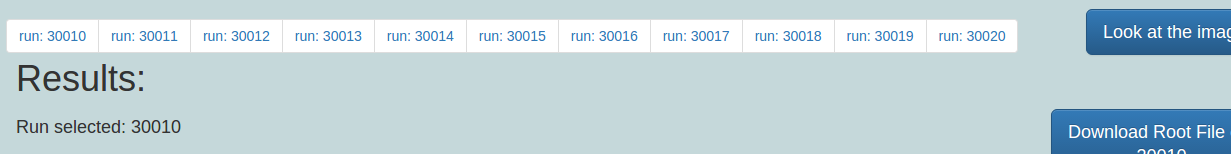
\includegraphics[scale=0.25]{WhichRunNavbar.png} 
\caption{By this "navbar" the user can choose the run results to show}
\end{figure}

This navbar is in fixed position related to the screen, and can be dragged by the user to allow him to decide where put it.

\item "Download Root File of: nnnn" is a button that allows to user to download the semi-processed file .root with some output information regarding the computation.

\item "Back to Home" gives the user the opportunity to directly return to the homepage. 

\item "Back to Home" and "Look at the images" are in a fixed position on the screen: also if the user scrolls down or up the screen he is always able to see these buttons.    

\end{enumerate}
The page that shows in an organized way the images that gAn produces in output. The following image shows the new appearance of the page:



\begin{figure}[H]
\centering
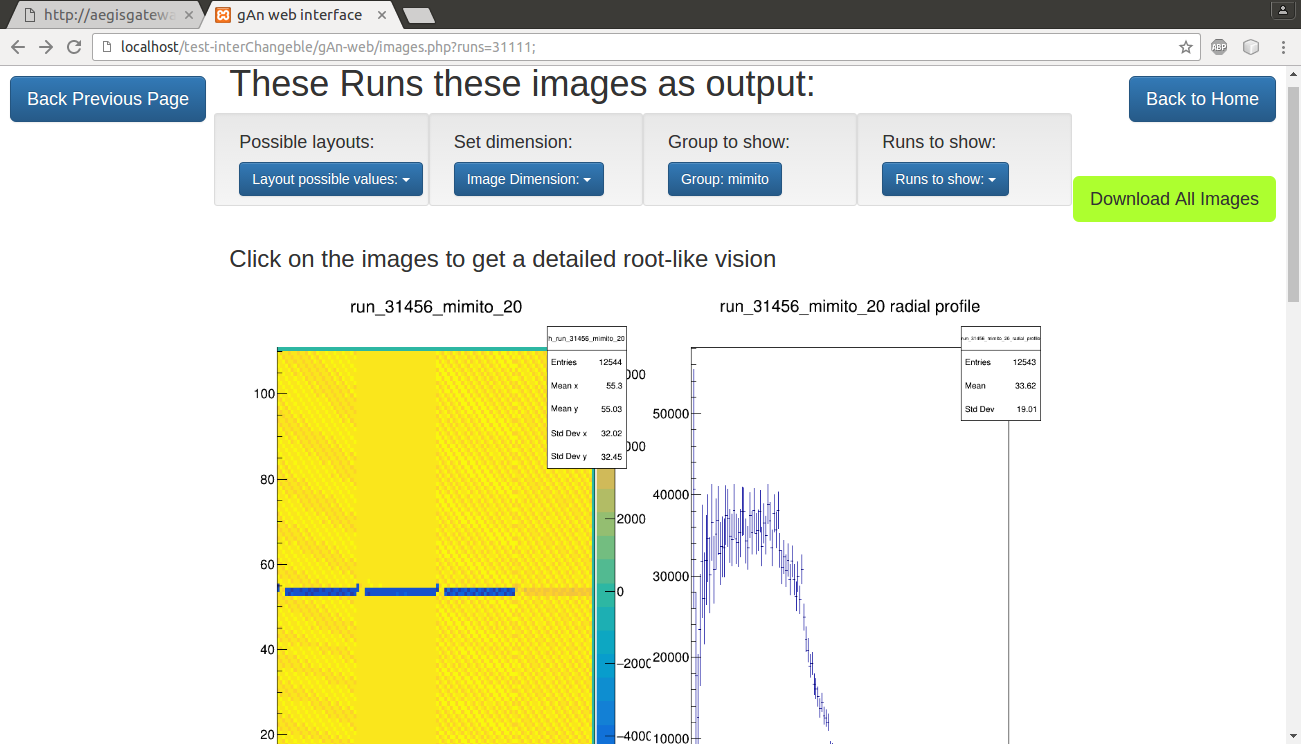
\includegraphics[scale=0.25]{AllImagesPage.png} 
\caption{This page shows all the images that gAn produces in output}
\end{figure}


Modifications:
\begin{enumerate}

\item The dropdown menu "Runs to show" allows the user to select only the images produced by a single run (by default the system shows the images related to all the runs). The users widely use this option, because in this way they can compare images extrapolated in the same way but related with runs with different configurations.

\item "Download All Images" allows the user to download by a single click all the images related to the execution. The late design introduces this requirement because commonly the users want to download the images using the right click of the mouse and the browser's button "Save Image As". In this way this process is faster and easier.

\item The buttons "Back to Previous page" and "Back to Home" are links towards the textual output page and the homepage. They are in fixed position.

\item By clicking on the image the user reaches a page that shows the image in full screen, but not in a static format: the image is dynamically accessible like shown in the following images:

\begin{figure}[H]
\centering
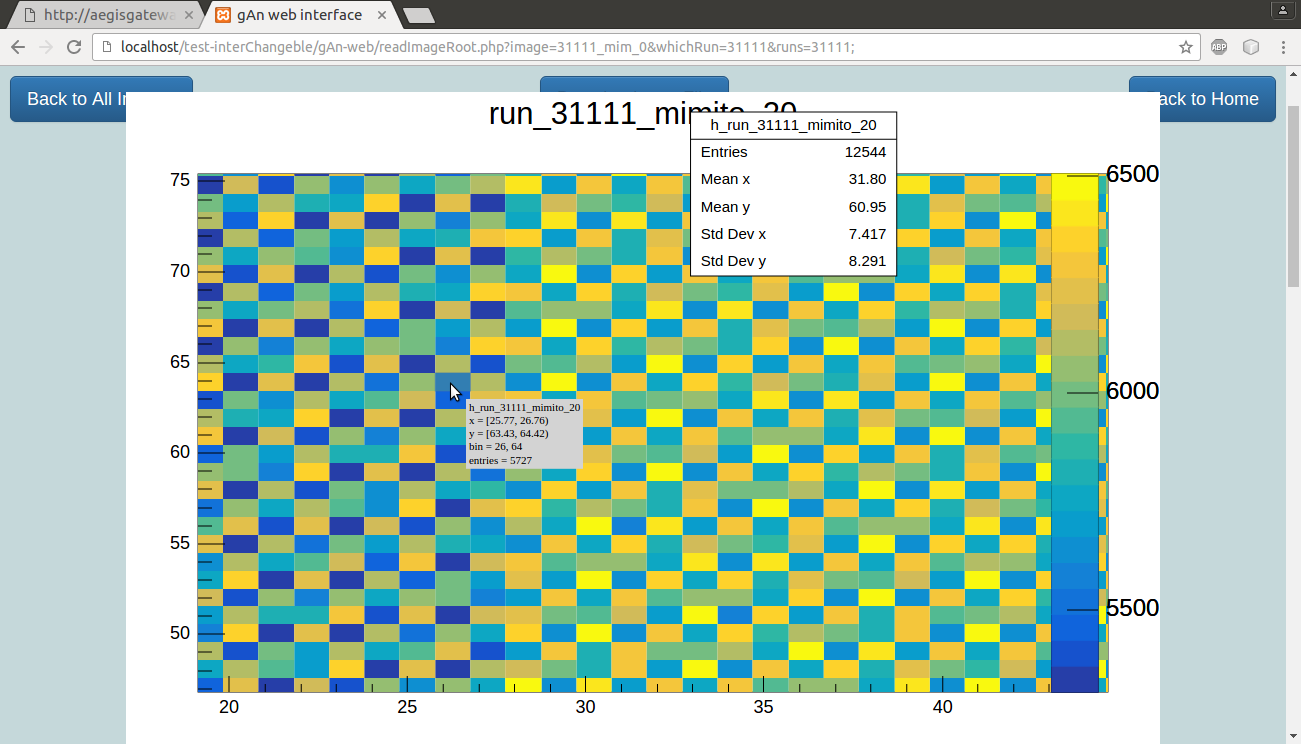
\includegraphics[scale=0.25]{RootLikeImage2.png} 
\caption{Moving the cursor the system shows the value of this histogram in the selected point}
\end{figure}



\begin{figure}[H]
\centering
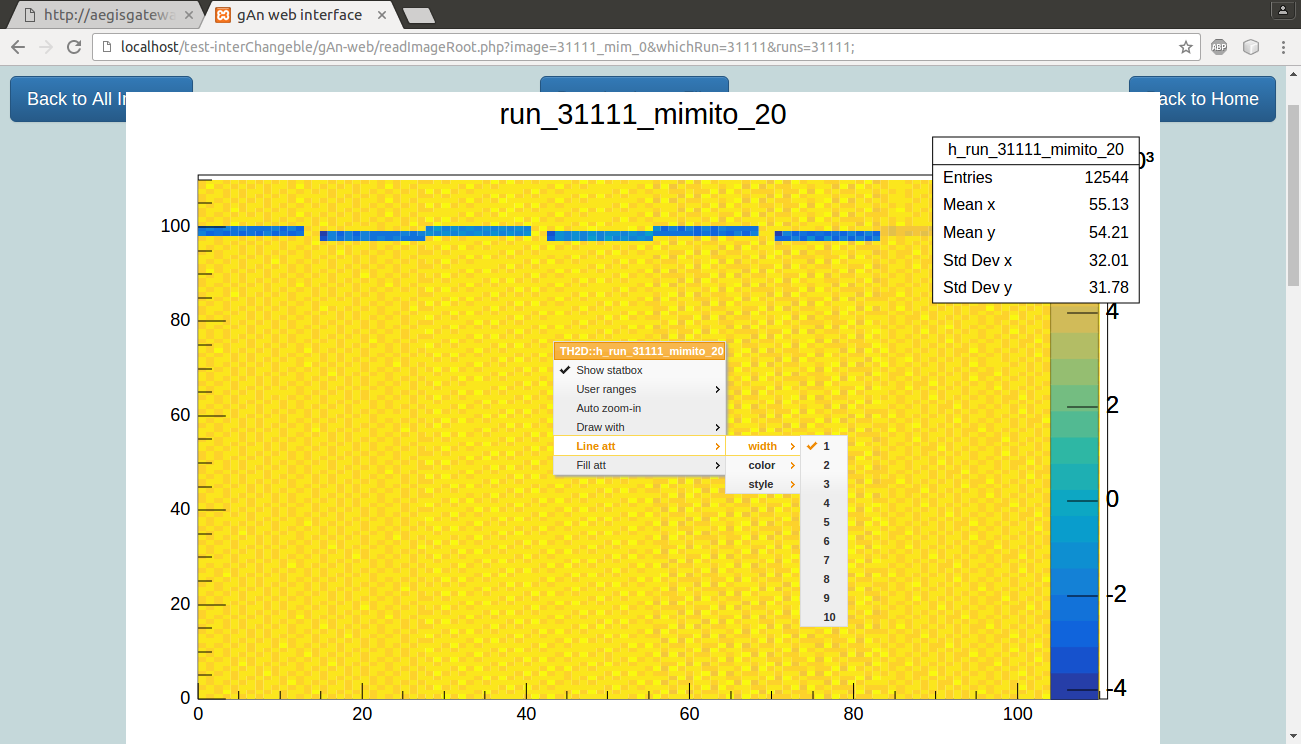
\includegraphics[scale=0.25]{RootLikeImage.png} 
\caption{The user can modify numerous settings in the generated image}
\end{figure}

\begin{figure}[H]
\centering
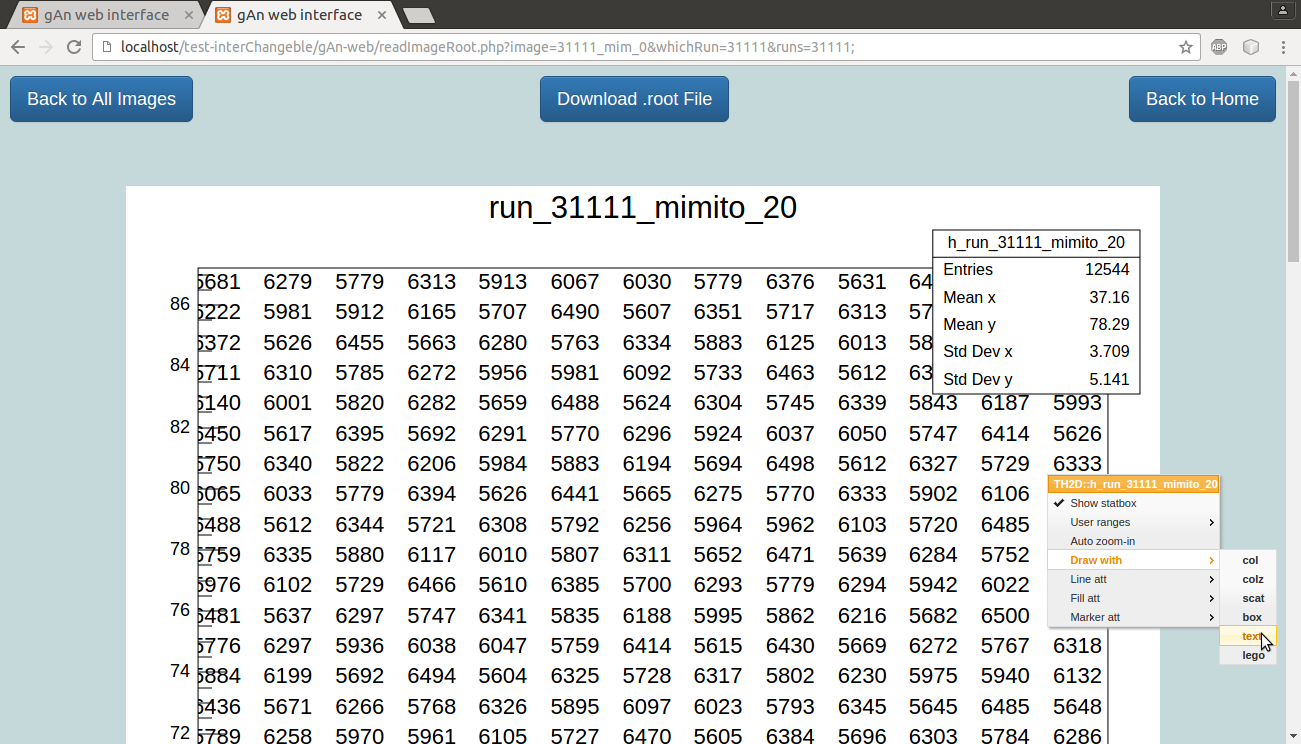
\includegraphics[scale=0.25]{RootLikeImage3.png} 
\caption{The user can show the histogram not only in traditional format, but also in a numerical format where the numbers are the value of the function in their position}
\end{figure}

\begin{figure}[H]
\centering
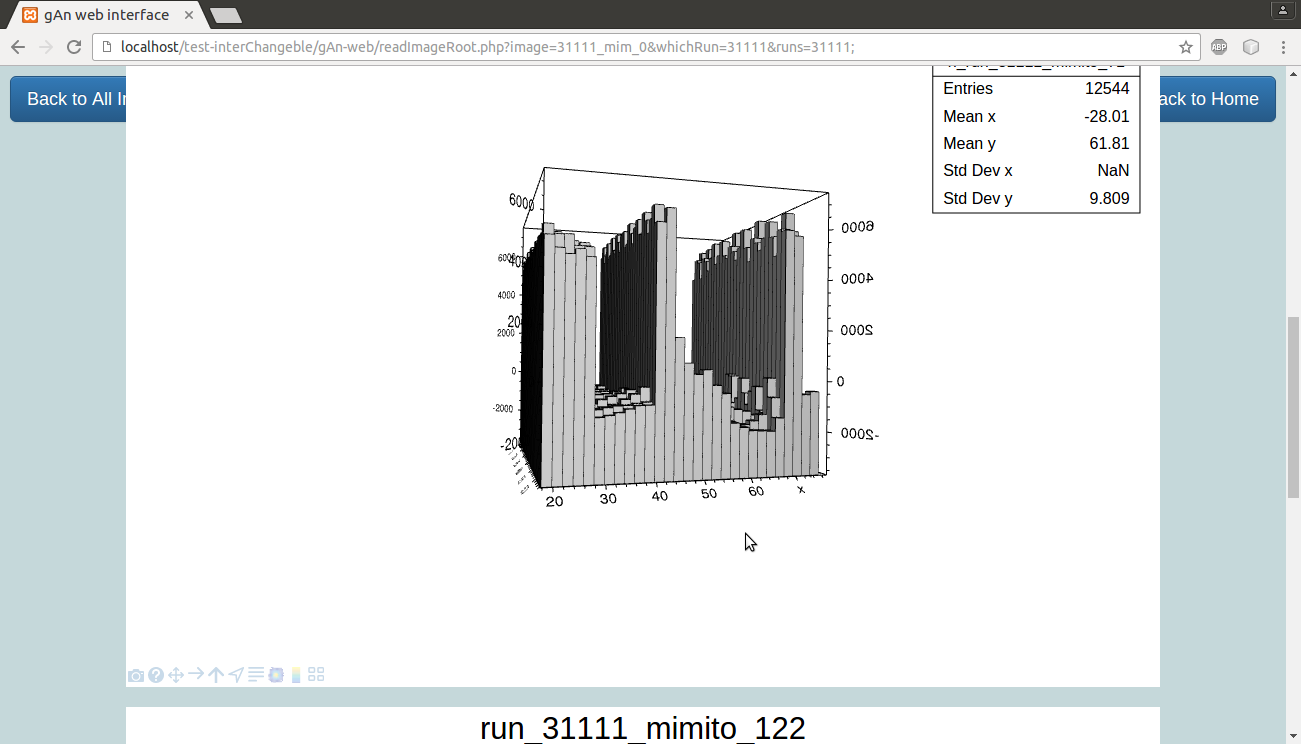
\includegraphics[scale=0.25]{RootLikeImage4.png} 
\caption{Another solution is to generate a 3d image in lego-style of the histogram}
\end{figure}


 
\end{enumerate}


\subsection{Added pages}

Some pages in the late version are completely new, because they implement new functionalities.

The first new page that the user sees is the login page. It is very simple, it doesn't authenticate a single user, but asks only the password of the office. This basic system of authentication aims simply to ensure that only the people that works in AEgIS experiment can use this software.

Following the login page image:

\begin{figure}[H]
\centering
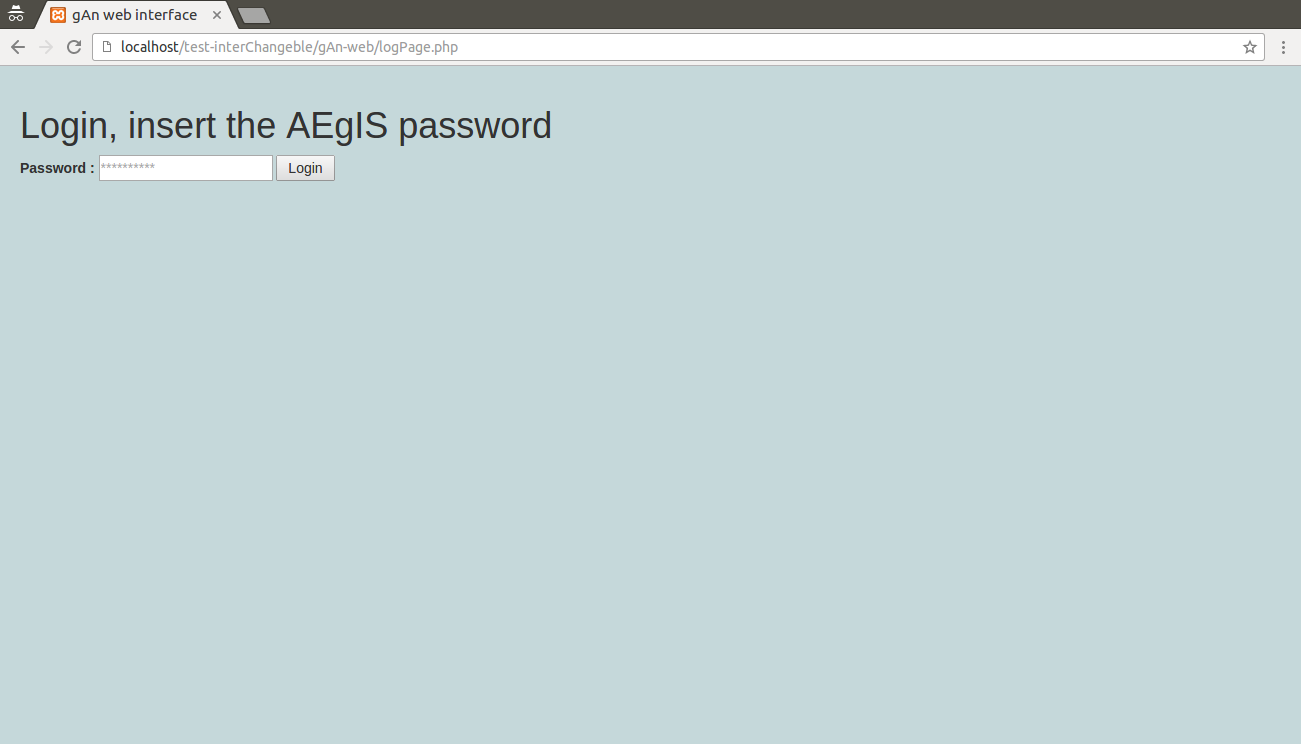
\includegraphics[scale=0.25]{Login.png} 
\caption{Simple login page}
\end{figure}

In the late version there is also the opportunity for the user to choose which branch of gAn and which version of Root Framework to use to execute the program. The pages that the user can user are quite similar, and quite simple. The user must use dropdown menus to make these choices, and there is always a default safe choice (the system remembers the last working version of Root and the last working branch of gAn), so it is impossible make errors or inconsistent choices. 

Following there are some screen-shots of these pages

\begin{figure}[H]
\centering
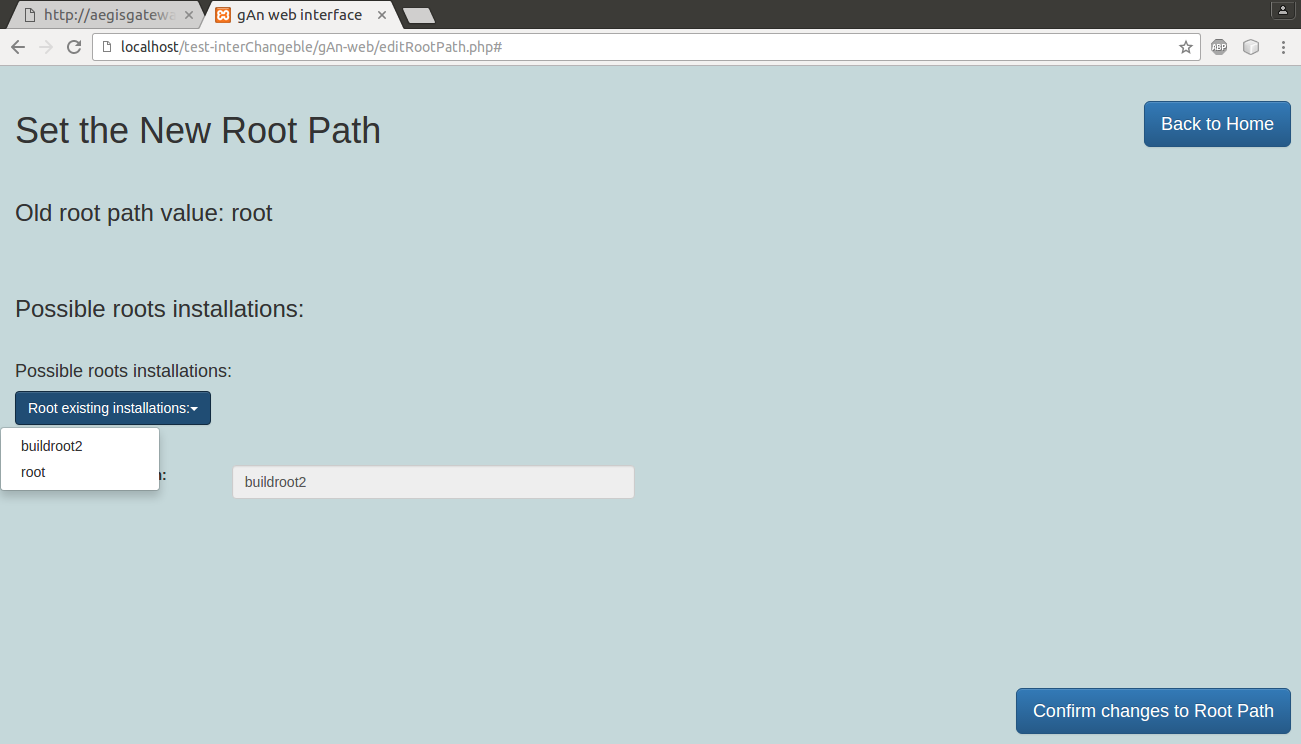
\includegraphics[scale=0.25]{RootVersionChoice.png} 
\caption{Page where the user can choose the Root version to use}
\end{figure}
 
 
\begin{figure}[H]
\centering
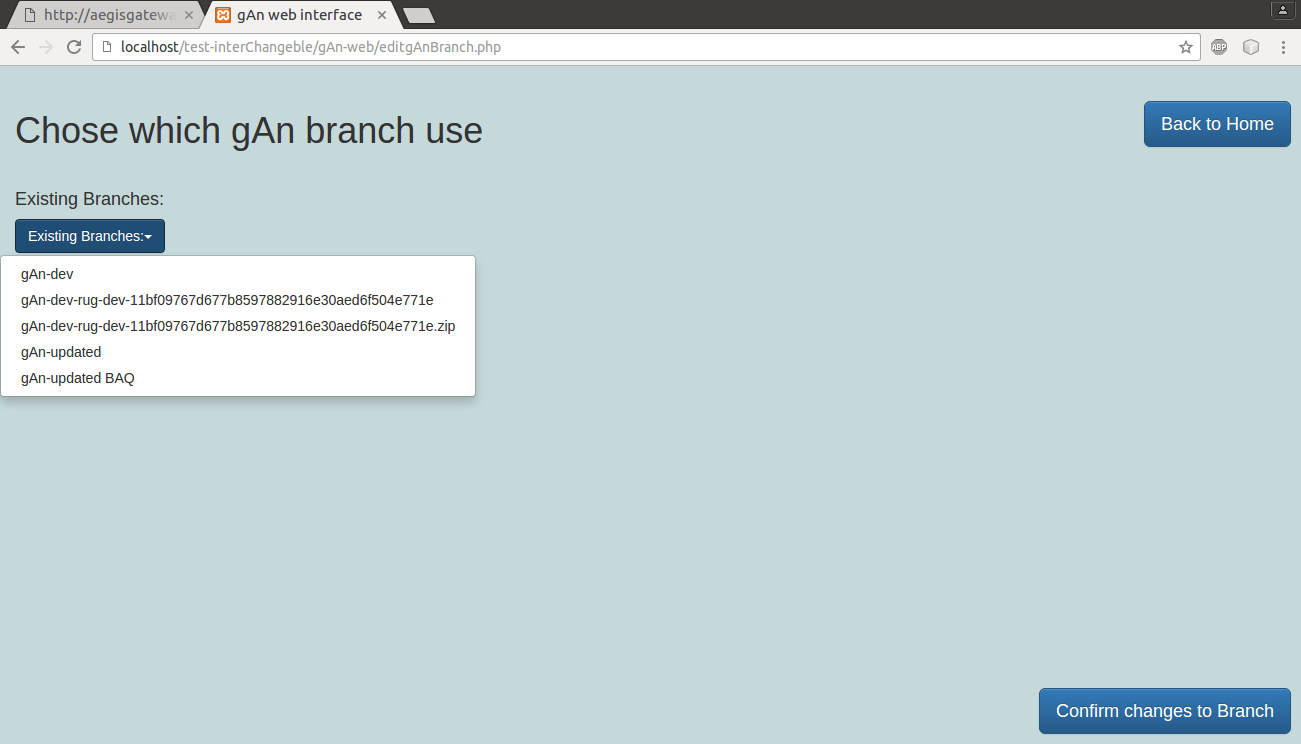
\includegraphics[scale=0.25]{ChoosegAnBranch.png} 
\caption{Page where the user can choose the Root version to use}
\end{figure}
